%=== CHAPTER FIVE (5) ===
%=== Discussion ===

\chapter{Integration Scenarios}
\section{Overview of Real-Time Integration}
This section provides a detailed overview of the real-time integration process between SAP S/4HANA, SAP CPI, and Salesforce, focusing on how data synchronization is achieved across these systems. The iFlow is specifically designed to facilitate the automated transfer of business-critical data, such as Business Partners (BP), from SAP S/4HANA to Salesforce, ensuring consistency and accuracy across platforms.

The integration process is structured into three key phases, each thoroughly examined to illustrate its role in the data exchange. These phases include data extraction and transmission from SAP S/4HANA, transformation and processing within SAP CPI, and API-based ingestion into Salesforce.

To enhance understanding, visual aids such as sequence diagrams, process flow charts, and screenshots are included. These illustrations help bridge technical explanations with real-world implementation, providing a clear representation of how data moves through the integration framework.

\subsection{Step 1: Business Partner Creation in SAP S/4HANA}

The integration process begins with the creation of a Business Partner (BP) in SAP S/4HANA, which serves as the foundation for maintaining customer and vendor records. SAP employs the BP concept to consolidate and streamline master data management, enabling seamless synchronization between SAP S/4HANA and external systems such as Salesforce.

\subsubsection{Accessing the Business Partner Transaction}
To create a new BP, users must navigate to the Business Partner (BP) transaction code in SAP S/4HANA:

\begin{enumerate}
    \item Open the SAP GUI and enter the transaction code \textbf{BP} in the command field.

    \begin{figure}[H]
    \centering
    \fbox{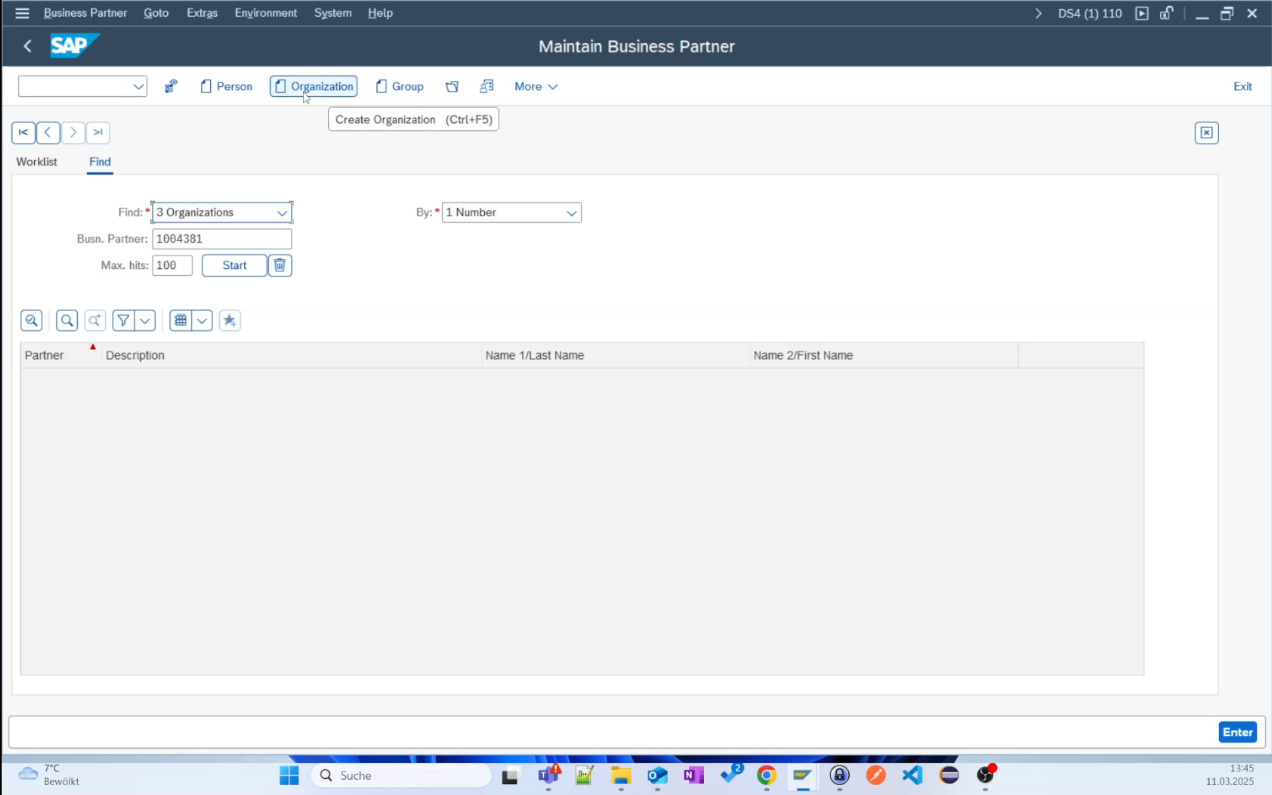
\includegraphics[width=0.8\textwidth]{Chapter5/Pictures/BP_Tcode.png}}
    \caption{Maintaining Business Partner in SAP S/4HANA}
    
    \end{figure}


    
    \item Press \textbf{Enter} to access the Business Partner maintenance screen.
\end{enumerate}



\subsubsection{Defining the Business Partner Role}
The BP framework in SAP S/4HANA allows the assignment of multiple roles to a single entity. To establish a customer relationship, the following steps are required:

\begin{enumerate}
    \item Click on the \textbf{Create Organization} or \textbf{Create Person} option, depending on the type of business partner being created.
    \item In the role selection dropdown, choose \textbf{Customer} to define the BP as a customer.
\end{enumerate}


    \begin{figure}[H]
    \centering
    \fbox{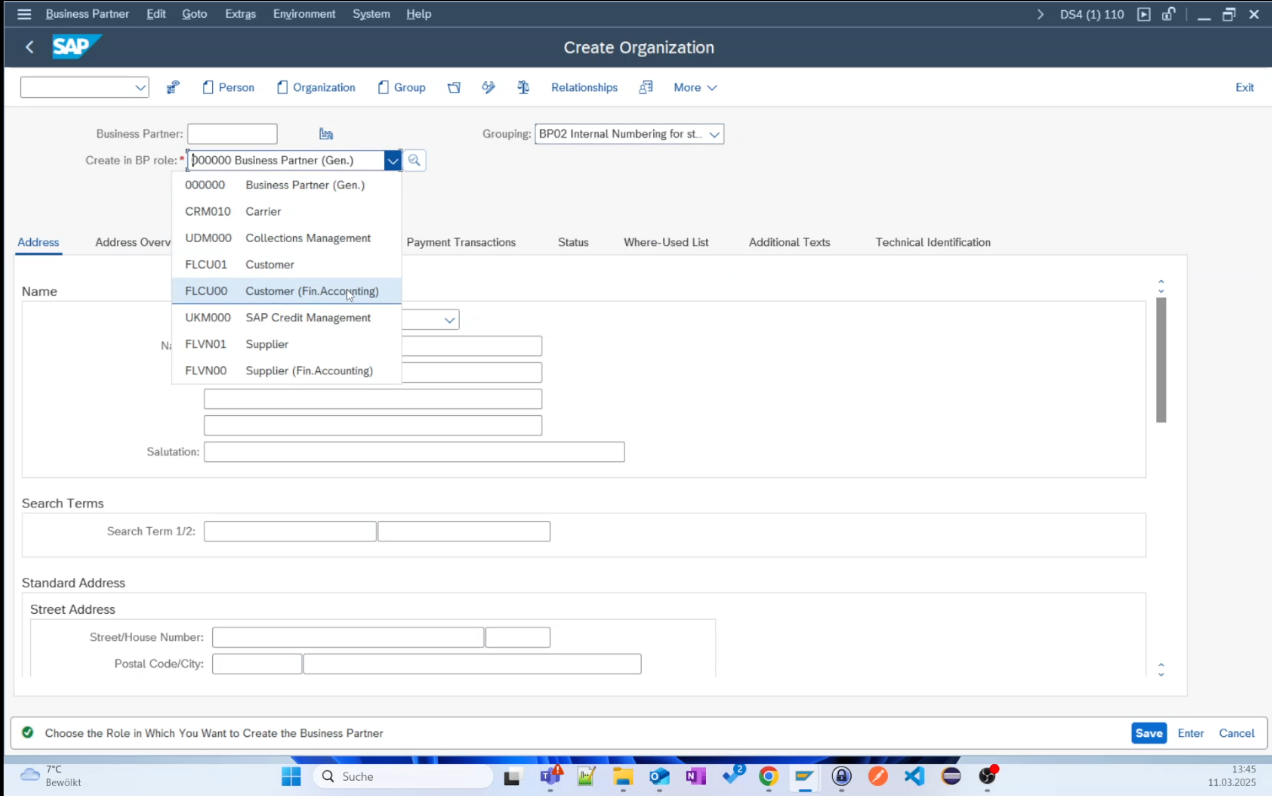
\includegraphics[width=0.8\textwidth]{Chapter5/Pictures/BP_Role.png}}
    \caption{Creating a Business Partner in SAP S/4HANA}
    
    \end{figure}

\subsubsection{Entering Business Partner Details}
After selecting the appropriate role, the system prompts the user to enter essential master data fields. These fields ensure the accurate classification and identification of the BP within SAP S/4HANA. The key required fields include:

\begin{itemize}
    \item \textbf{General Data:} Name, Address, Country, and Communication Details (e.g., Email, Phone).
    \item \textbf{Company Code Data:} Reconciliation Account and Payment Terms.
    \item \textbf{Sales and Distribution Data:} Sales Organization, Distribution Channel, Division, and Pricing Conditions.
\end{itemize}

Once all the required fields are populated, the BP record is saved and a unique Business Partner ID is generated. This ID serves as a reference for further processing and integration.


    \begin{figure}[H]
    \centering
    \fbox{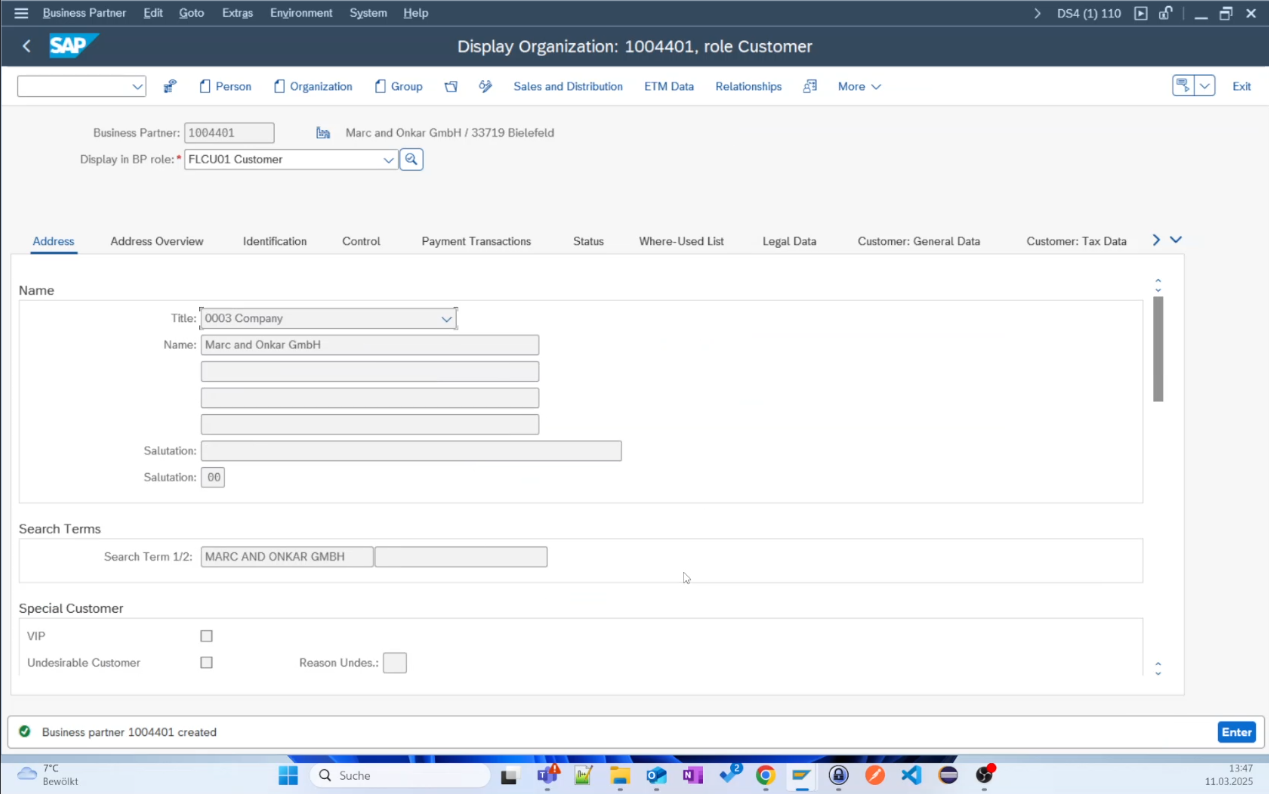
\includegraphics[width=0.8\textwidth]{Chapter5/Pictures/BP_generated.png}}
    \caption{Displaying Business Partner in SAP S/4HANA}
    
    \end{figure}

\subsubsection{Business Partner Readiness for Integration}
With the BP successfully created, it is now available for outbound integration to Salesforce via SAP CPI. The next step involves triggering the data transfer through IDoc generation, which is covered in the subsequent section.


\subsection{Step 2: iFlow Execution in SAP CPI}

Once the Business Partner (BP) is created in SAP S/4HANA, the next step involves the execution of the integration flow (iFlow) within SAP Cloud Platform Integration (CPI) to transfer the BP data to Salesforce. The iFlow acts as a middleware process, ensuring that the data is properly mapped, transformed, and securely transmitted between SAP and Salesforce.

\subsubsection{Triggering the iFlow Execution}
The iFlow in SAP CPI can be triggered in two ways:
\begin{itemize}
    \item \textbf{Scheduled Execution:} The iFlow can be configured to run at predefined intervals, ensuring periodic synchronization between SAP S/4HANA and Salesforce.
    \item \textbf{Immediate Execution:} The iFlow can be triggered manually by deploying it within SAP CPI, initiating the data transfer in real time.
\end{itemize}

For real-time synchronization, an immediate trigger is preferred, which is initiated when the iFlow is deployed.

\subsubsection{Executing the iFlow in SAP CPI}
To execute the iFlow manually, the following steps must be performed:

\begin{enumerate}
    \item \textbf{Access SAP CPI:}
    Log in to the SAP Integration Suite via the SAP BTP cockpit.
    
    \item \textbf{Navigate to the iFlow:}
    \begin{itemize}
        \item Go to the Design workspace.
        \item Locate the integration package containing the iFlow named "Replicate Account from SAP S/4HANA to Salesforce."
    \end{itemize}
    
    \begin{figure}[H]
    \centering
    \fbox{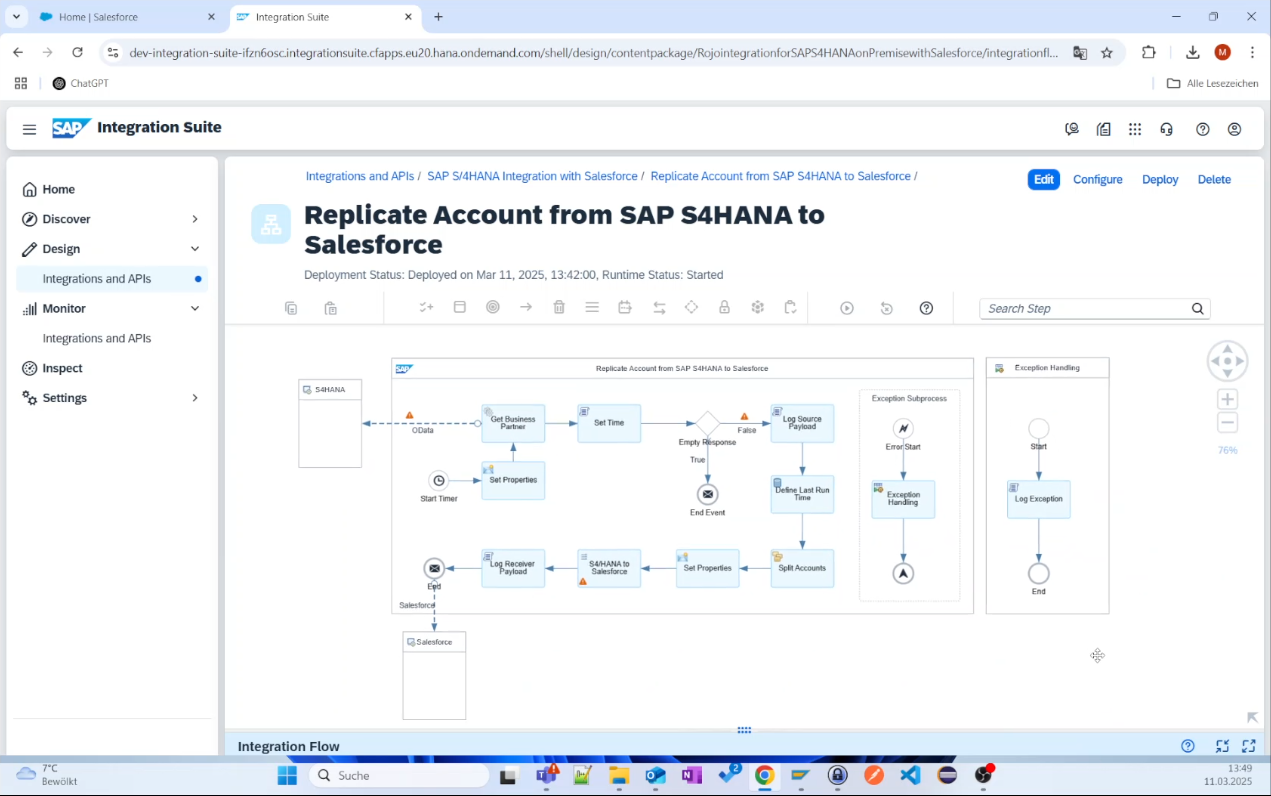
\includegraphics[width=0.8\textwidth]{Chapter5/Pictures/CPI_Locate.png}}
    \caption{Integration Flow for Replicating Accounts from SAP S/4HANA to Salesforce}
    
    \end{figure}
    
    \item \textbf{Deploy the iFlow:}
    \begin{itemize}
        \item Select the iFlow.
        \item Click on the Deploy button to initiate execution.
    \end{itemize}


    \item \textbf{Monitor the Execution Status:}
    \begin{itemize}
        \item Navigate to the Monitor tab within SAP CPI.
        \item Open Message Monitoring to check the processing status of the deployed iFlow.
    \end{itemize}

        
    \begin{figure}[H]
    \centering
    \fbox{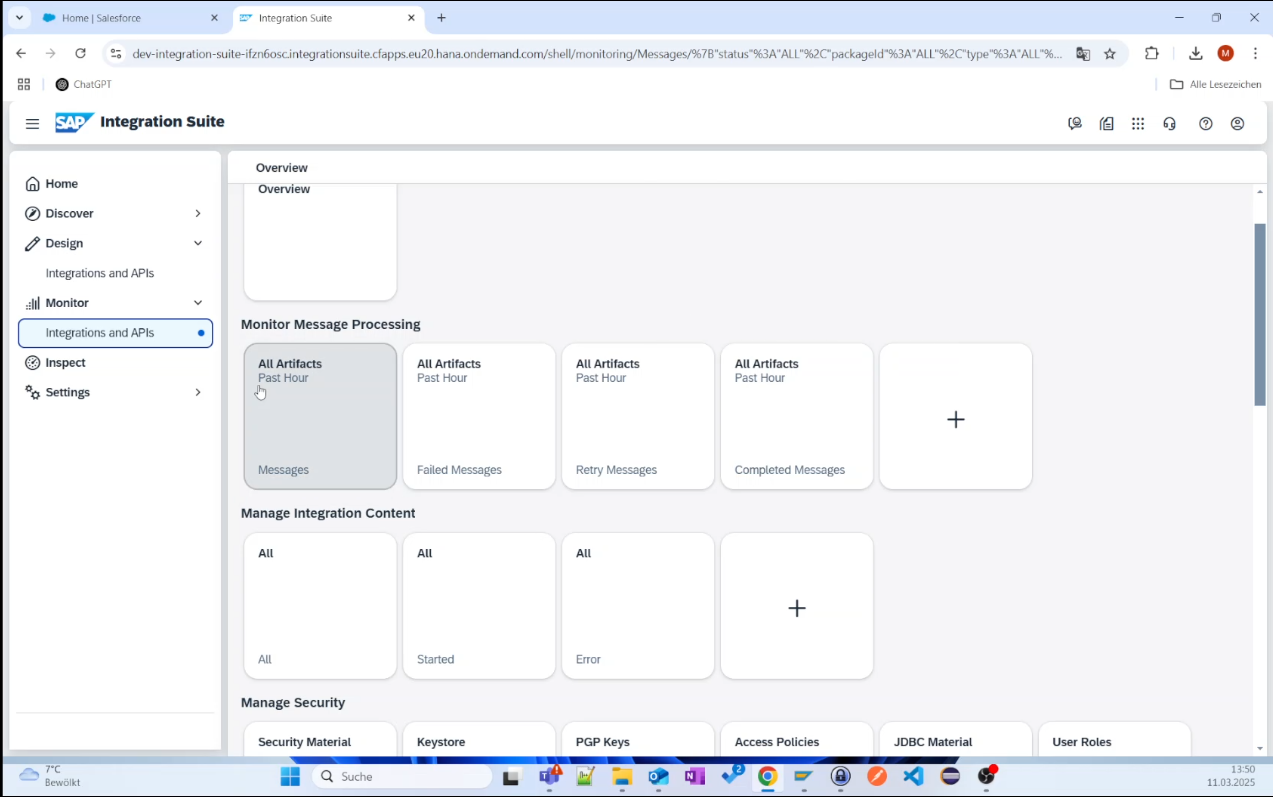
\includegraphics[width=0.8\textwidth]{Chapter5/Pictures/CPI_Mon.png}}
    \caption{Monitoring Message Processing in SAP BTP Integration Suite}
    
    \end{figure}

    \begin{figure}[H]
    \centering
    \fbox{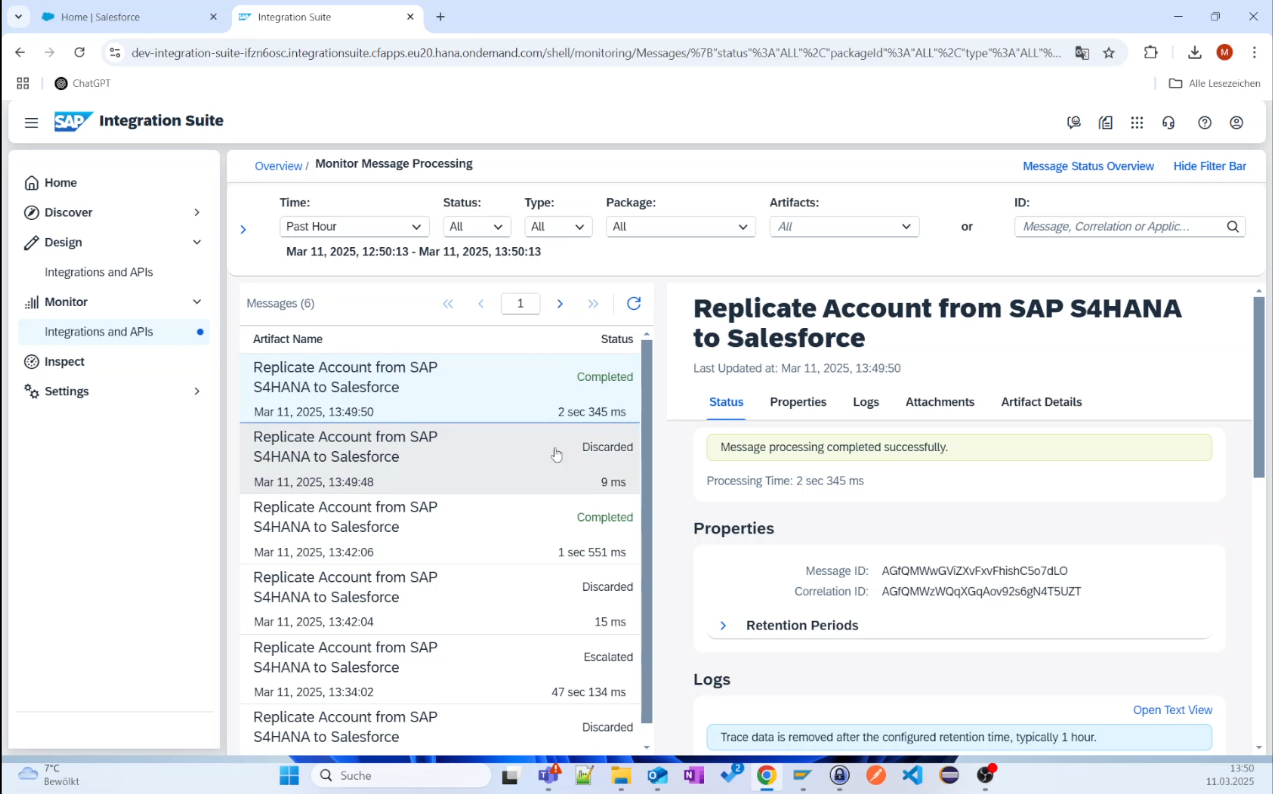
\includegraphics[width=0.8\textwidth]{Chapter5/Pictures/CPI_sucess.png}}
    \caption{Message Monitoring in SAP BTP Integration Suite}
    
    \end{figure}
    
    \item \textbf{Verify the Execution Results:}
    \begin{itemize}
        \item Look for a Success message in the message processing logs, indicating successful data transfer.
        \item Open the detailed logs to review the exact data payload transferred from SAP S/4HANA to Salesforce.
    \end{itemize}
\end{enumerate}

    \begin{figure}[H]
    \centering
    \fbox{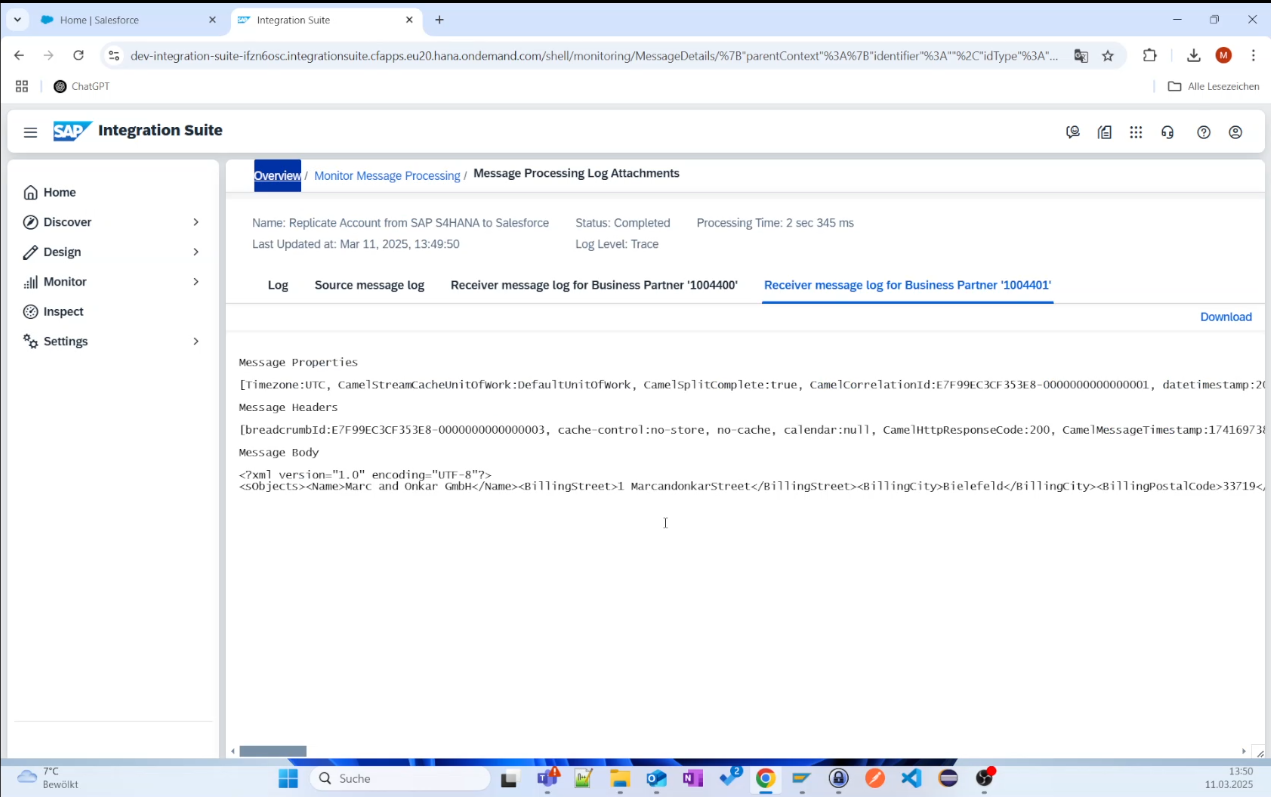
\includegraphics[width=0.8\textwidth]{Chapter5/Pictures/CPI_Verify.png}}
    \caption{Message Processing Log in SAP BTP Integration Suite}
    
    \end{figure}

This step ensures that the iFlow is successfully executed, facilitating seamless data replication from SAP S/4HANA to Salesforce. The next section explores potential error scenarios and strategies for resolving common integration challenges.

\subsection{Step 3: Login to Salesforce and Display the Transferred Business Partner as an Account}

After the successful execution of the iFlow in SAP CPI, the next step involves verifying the data transfer by logging into Salesforce and locating the Business Partner (BP) record, which is stored as an Account in Salesforce. This step ensures that the integration process has completed successfully and that the transferred data is available for business operations.

\subsubsection{Accessing Salesforce}
To verify the transferred data in Salesforce, the following steps should be performed:

\begin{enumerate}
    \item Open a web browser and navigate to the Salesforce login page at \texttt{https://login.salesforce.com}.
    \item Enter the Salesforce credentials (username and password) and click on the Login button.
    \item Once logged in, navigate to the Sales Cloud dashboard or use the global search bar to locate the transferred record.
\end{enumerate}

\subsubsection{Locating the Transferred Business Partner}
Since SAP S/4HANA's Business Partner is mapped to the Account entity in Salesforce, the transferred data can be accessed as follows:

\begin{enumerate}
    \item Click on the \textbf{Accounts} tab in the Salesforce navigation menu.

    \begin{figure}[H]
    \centering
    \fbox{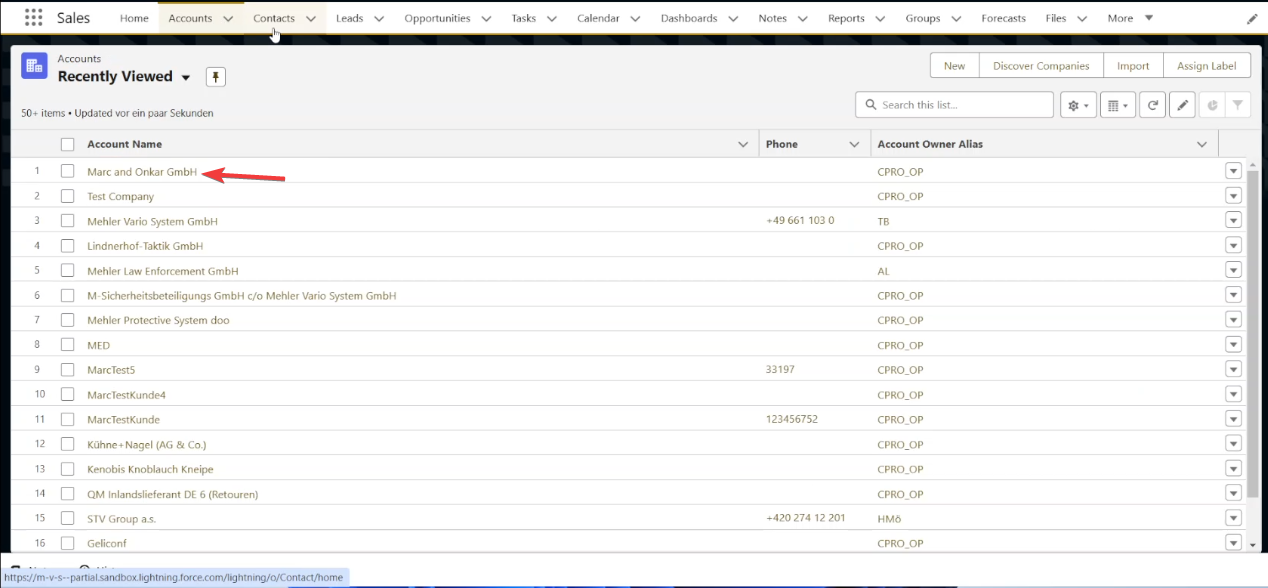
\includegraphics[width=0.8\textwidth]{Chapter5/Pictures/SF_ACC_ED.png}}
    \caption{Salesforce Account List View}
    
    \end{figure}
    
    \item In the search bar, enter the Business Partner ID or name that was transferred from SAP S/4HANA.
    \item Click on the corresponding Account record to view its details.
\end{enumerate}

    \begin{figure}[H]
    \centering
    \fbox{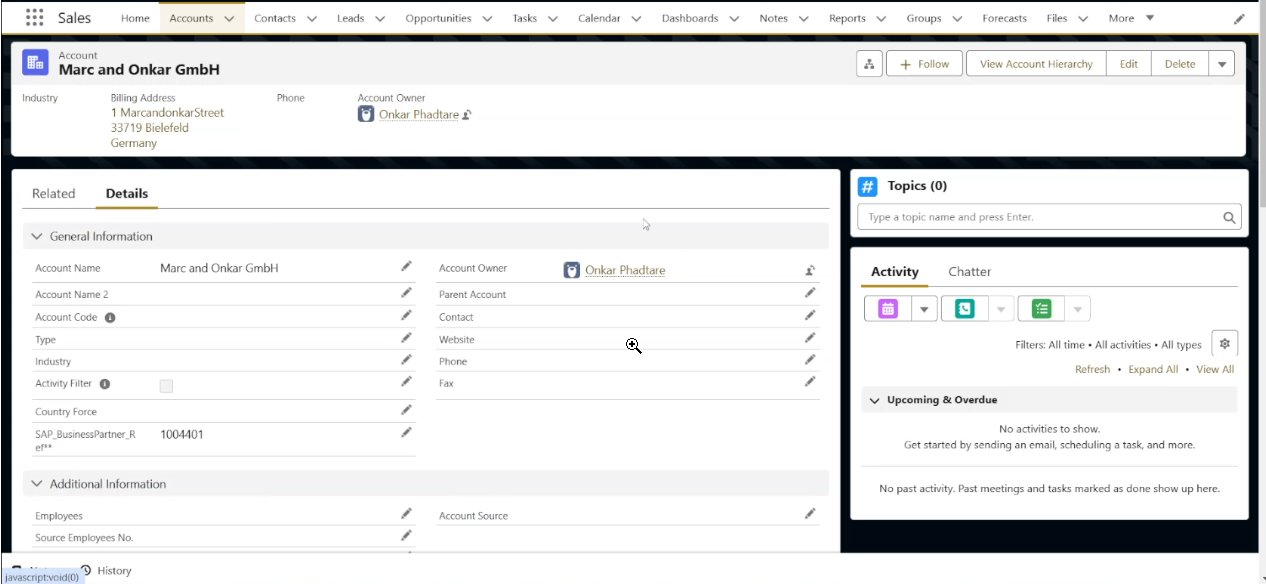
\includegraphics[width=0.8\textwidth]{Chapter5/Pictures/SF_Fields_ED.png}}
    \caption{Salesforce Account Details Page}
    
    \end{figure}

\subsubsection{Validating Data Accuracy}
Once the Account record is opened, it is essential to verify that the data has been correctly transferred. Key fields that should be checked include:

\begin{itemize}
    \item \textbf{Account Name:} Should match the Business Partner Name in SAP S/4HANA.
    \item \textbf{Address Details:} Street, City, Postal Code, and Country should be correctly mapped.
    \item \textbf{Industry and Classification:} If applicable, ensure these attributes have been accurately assigned.
    \item \textbf{Sales Information:} Sales Group, Account Owner, and other relevant fields should be reviewed.
\end{itemize}

If any discrepancies are found, the integration logs in SAP CPI should be analyzed to determine if there were mapping errors, missing fields, or issues related to data transformation.

\subsubsection{Handling Missing or Incorrect Data}
If the Business Partner record does not appear in Salesforce, or if critical data fields are missing, the following troubleshooting steps should be performed:

\begin{itemize}
    \item Verify that the iFlow execution in SAP CPI was successful and check the message logs.
    \item Check for any API errors in Salesforce under \textit{Setup} → \textit{API Usage Logs}.
    \item Ensure that the Salesforce user account has the necessary permissions to view the Account records.
    \item Re-run the iFlow in SAP CPI and monitor if the data transfer is successful.
\end{itemize}

This step confirms the successful integration of Business Partner records from SAP S/4HANA to Salesforce. By verifying the transferred data within the Salesforce Account entity, organizations can ensure that the synchronization process maintains data integrity and supports business operations. If errors or inconsistencies arise, further analysis of the iFlow execution and data transformation logs is required to rectify the issues.



\section{Error Scenario in iFlow Execution}

While the integration of SAP S/4HANA and Salesforce through SAP CPI ensures seamless data synchronization, failures in the iFlow execution can occur due to misconfigurations, expired credentials, or network-related issues. Understanding these failure scenarios is essential for troubleshooting and improving integration reliability. 

This section examines a controlled error scenario where an expired OAuth credential is deliberately used during Business Partner (BP) creation in SAP S/4HANA. The resulting iFlow failure is analyzed through message monitoring in SAP CPI.

\subsection{Intentional Error Injection: Expired OAuth Credentials}
To demonstrate an authentication failure scenario, an expired OAuth credential is intentionally used during the execution of the iFlow. The following steps outline the controlled setup:

\begin{enumerate}
    \item \textbf{Create a Business Partner in SAP S/4HANA:}  
    A new BP is created using transaction code \texttt{BP}, following the standard process outlined in Section 5.1.
    
    \item \textbf{Modify SAP CPI Credentials:}  
    The OAuth credentials stored in SAP CPI are deliberately replaced with an expired or incorrect client secret from the Salesforce Connected App.

    \begin{figure}[H]
    \centering
    \fbox{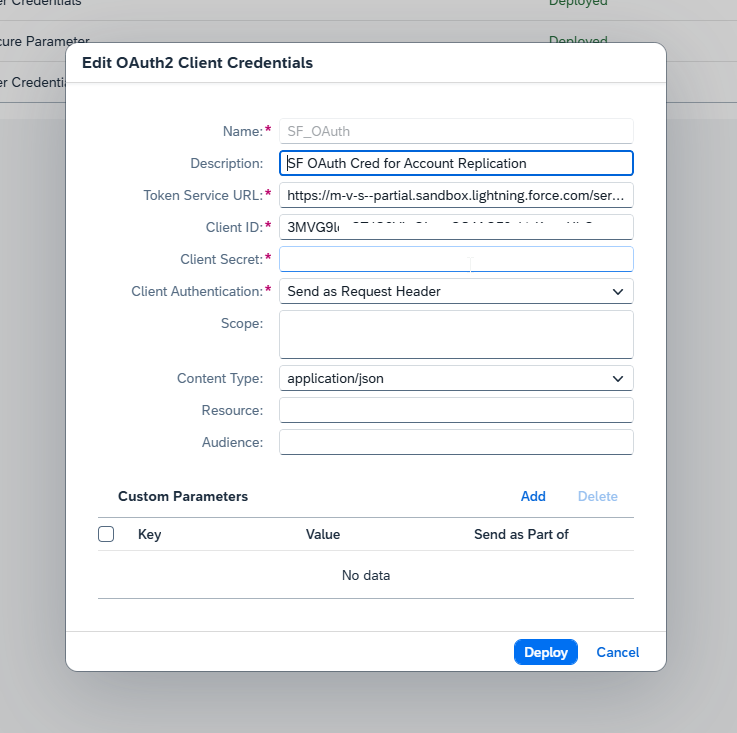
\includegraphics[width=0.8\textwidth]{Chapter5/Pictures/Fail_oauth.png}}
    \caption{OAuth2 Client Credentials Configuration in SAP Integration Suite}
    
    \end{figure}
    
    \item \textbf{Deploy the iFlow and Monitor Execution:}  
    The iFlow responsible for BP replication is deployed, initiating data transfer from SAP S/4HANA to Salesforce.
\end{enumerate}

\subsection{Failed Status in SAP CPI Monitor Tab}
After triggering the iFlow, the message monitoring dashboard in SAP CPI provides insights into the error encountered. The key observations include:

\begin{itemize}
    \item \textbf{Status:} The iFlow execution fails, displaying a "Failed" status in the Monitor tab.
    
    \begin{figure}[H]
    \centering
    \fbox{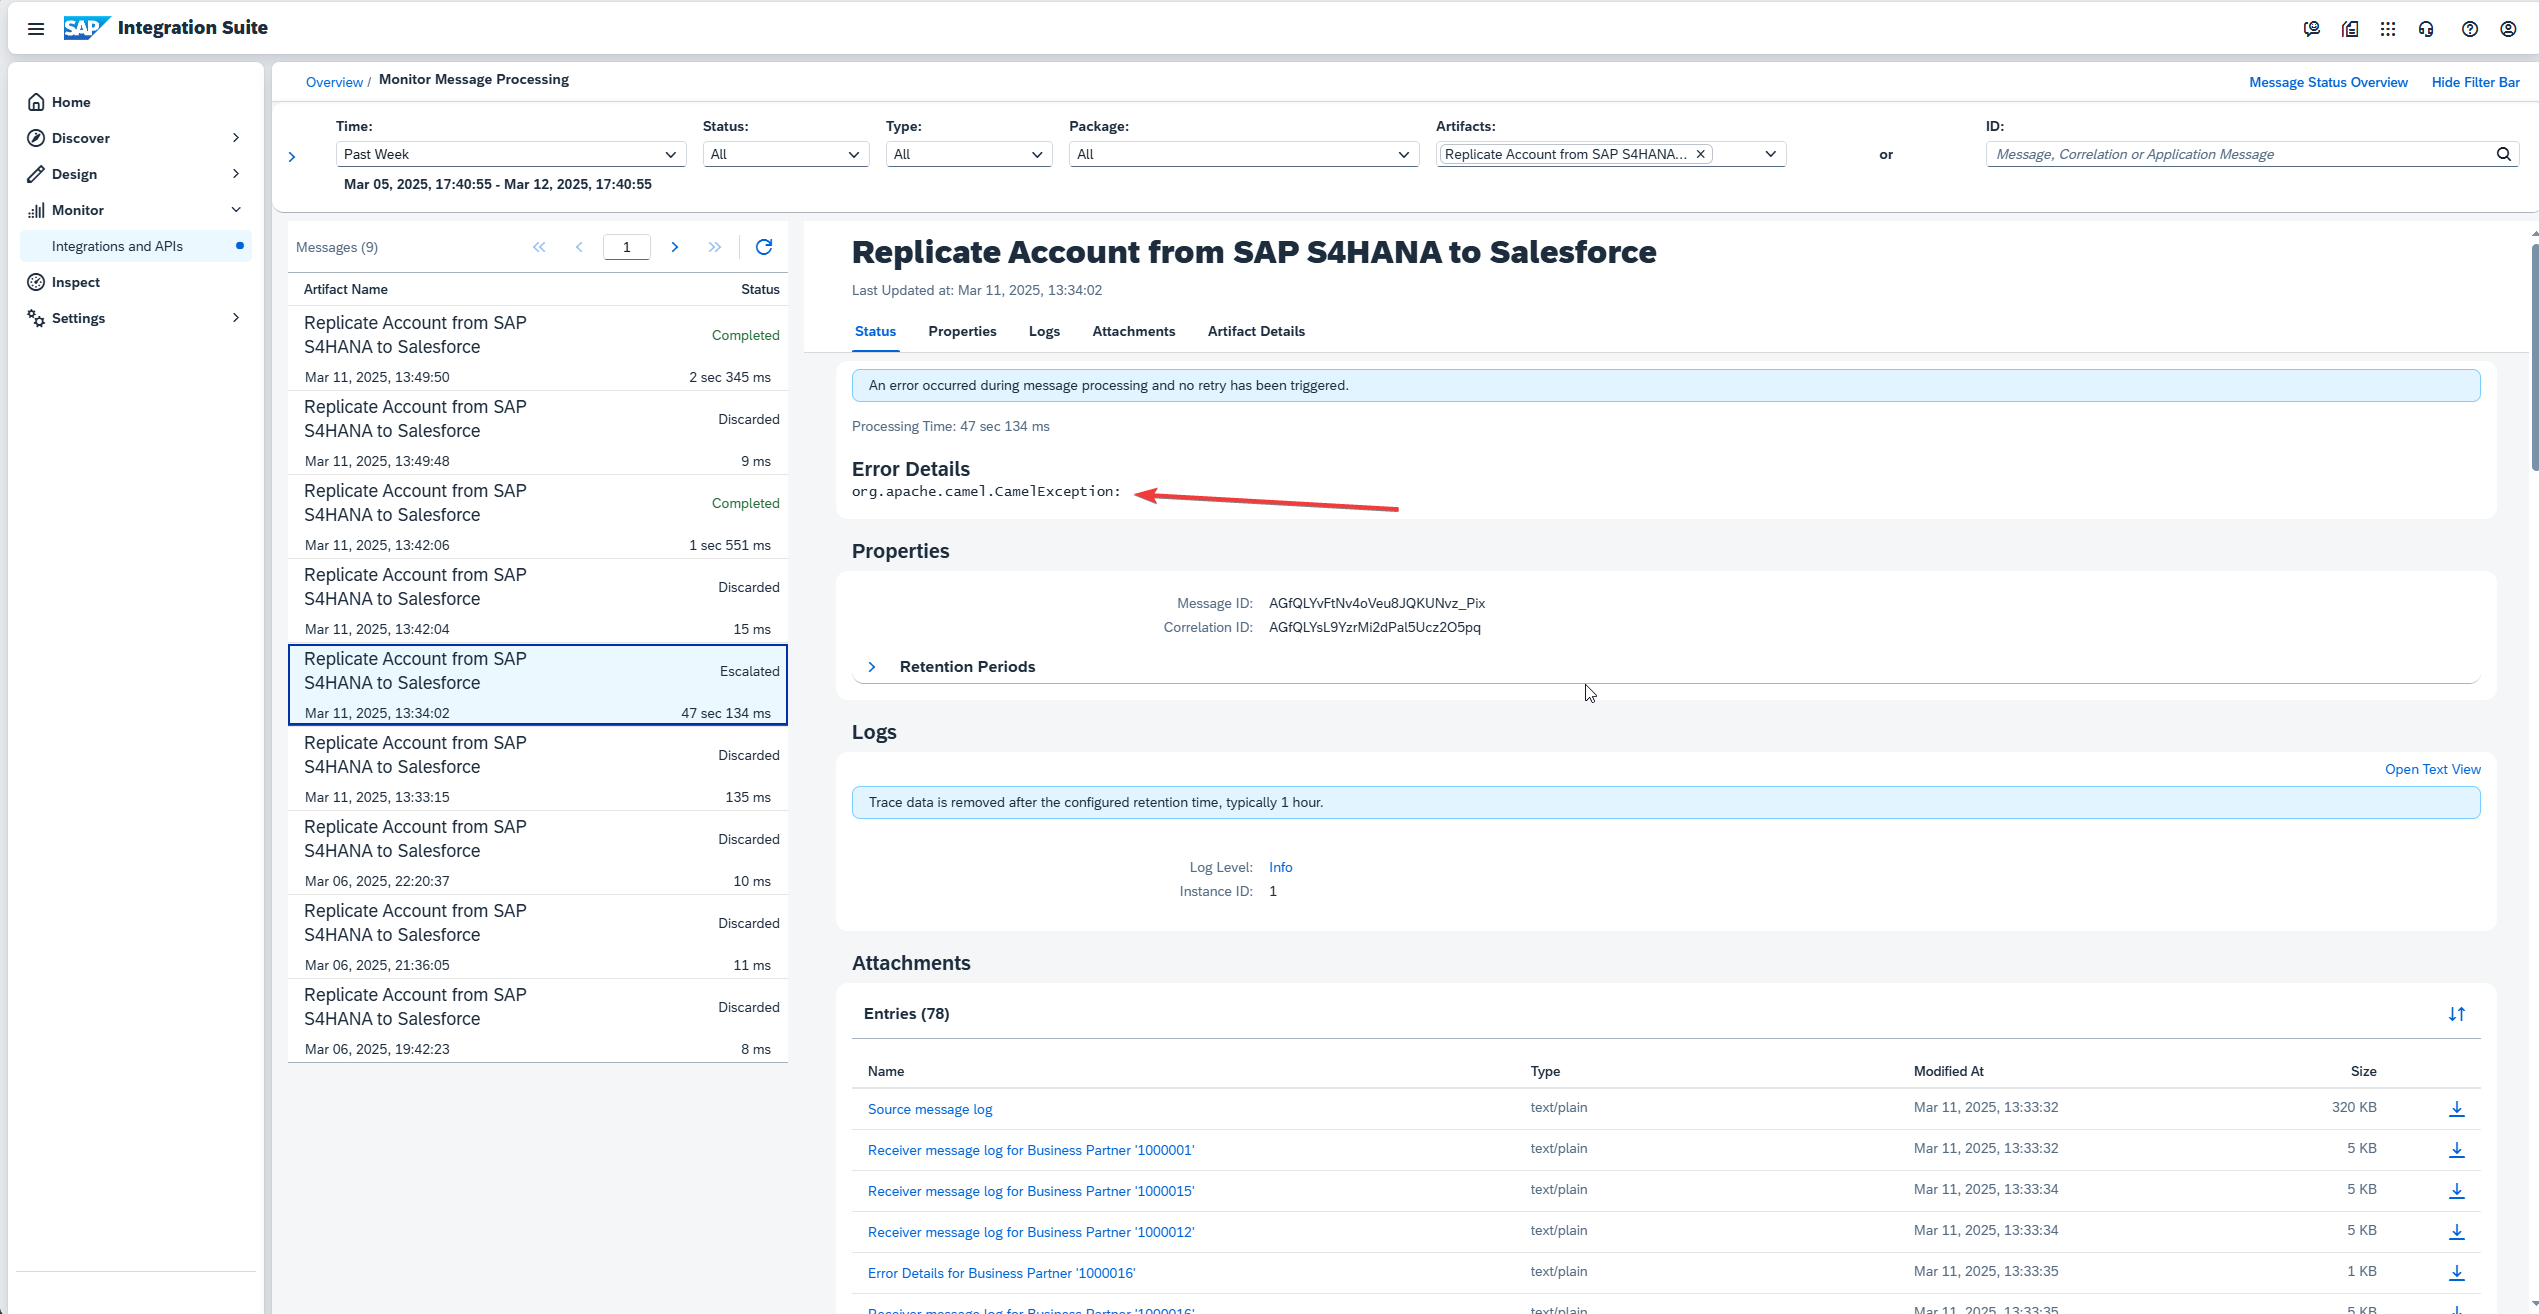
\includegraphics[width=0.8\textwidth]{Chapter5/Pictures/fail_error.png}}
    \caption{Message Processing Run in SAP BTP Integration Suite}
    
    \end{figure}
    
    \item \textbf{Error Message:} The logs indicate an authentication failure due to expired or incorrect OAuth credentials.
    \item \textbf{Timestamp and Log Details:} The failure occurs at the authentication step, preventing further processing of the BP data.
    
\end{itemize}

\subsection{Analyzing the Error Logs}
To investigate the root cause, the following log files in SAP CPI are examined:
    \begin{figure}[H]
    \centering
    \fbox{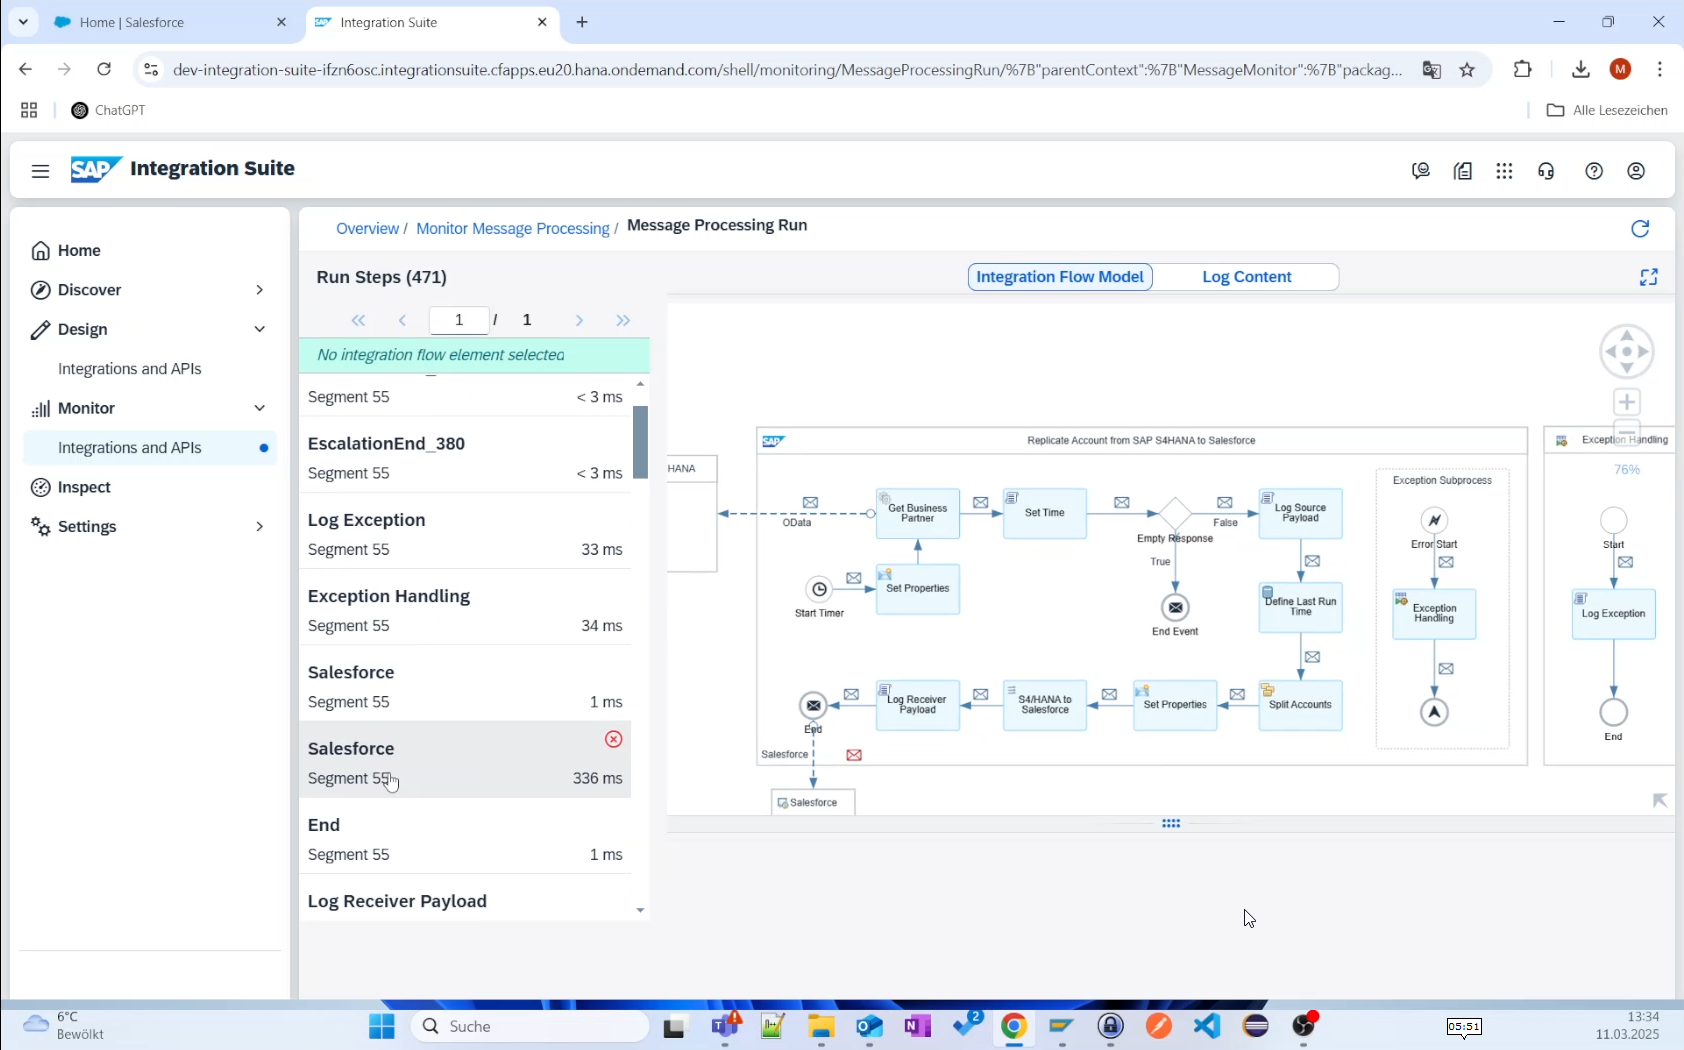
\includegraphics[width=0.8\textwidth]{Chapter5/Pictures/Fail_log.png}}
    \caption{Error Log in SAP BTP Integration Suite}
    
    \end{figure}
\begin{itemize}
    \item \textbf{Integration Message Logs:} Provide details on failed API authentication.
    \item \textbf{OAuth Token Validation:} Indicates an invalid or expired access token.
    \item \textbf{Salesforce API Logs:} Can be checked under \textit{Setup → API Usage Logs} in Salesforce to confirm rejected authentication requests.
\end{itemize}

\subsection{Corrective Measures}
To resolve this issue and ensure successful execution, the following corrective actions must be implemented:

\begin{itemize}
    \item \textbf{Regenerate OAuth Credentials:} Obtain a new access token from the Salesforce Connected App.
    \item \textbf{Update SAP CPI Credentials:} Replace the expired credentials in the security material of SAP CPI.
    \item \textbf{Re-execute the iFlow:} Once the correct credentials are in place, redeploy the iFlow and monitor execution.
\end{itemize}


This error scenario highlights the critical role of proper authentication management in SAP CPI integrations. Expired OAuth credentials can disrupt real-time data synchronization, necessitating proactive monitoring and periodic credential updates. By leveraging SAP CPI’s message monitoring and Salesforce API logs, authentication failures can be swiftly diagnosed and corrected, ensuring seamless integration between SAP S/4HANA and Salesforce.



\section{Limitations of the Current Development}

While the integration between SAP S/4HANA and Salesforce using SAP CPI enables seamless data synchronization, several limitations exist within the current development. These limitations primarily relate to field mapping complexities, inadequate error messaging, and restricted access to trial environments. Understanding these challenges is crucial for improving the integration framework and addressing potential constraints in future implementations.

\subsection{Mapping Complexity in iFlow Development}
One of the significant challenges in the current integration setup is the extensive field mapping required between SAP S/4HANA and Salesforce. Due to differences in data structures and field names between the two systems, each data element must be carefully mapped to ensure successful data transformation and transfer.

    \begin{figure}[H]
    \centering
    \fbox{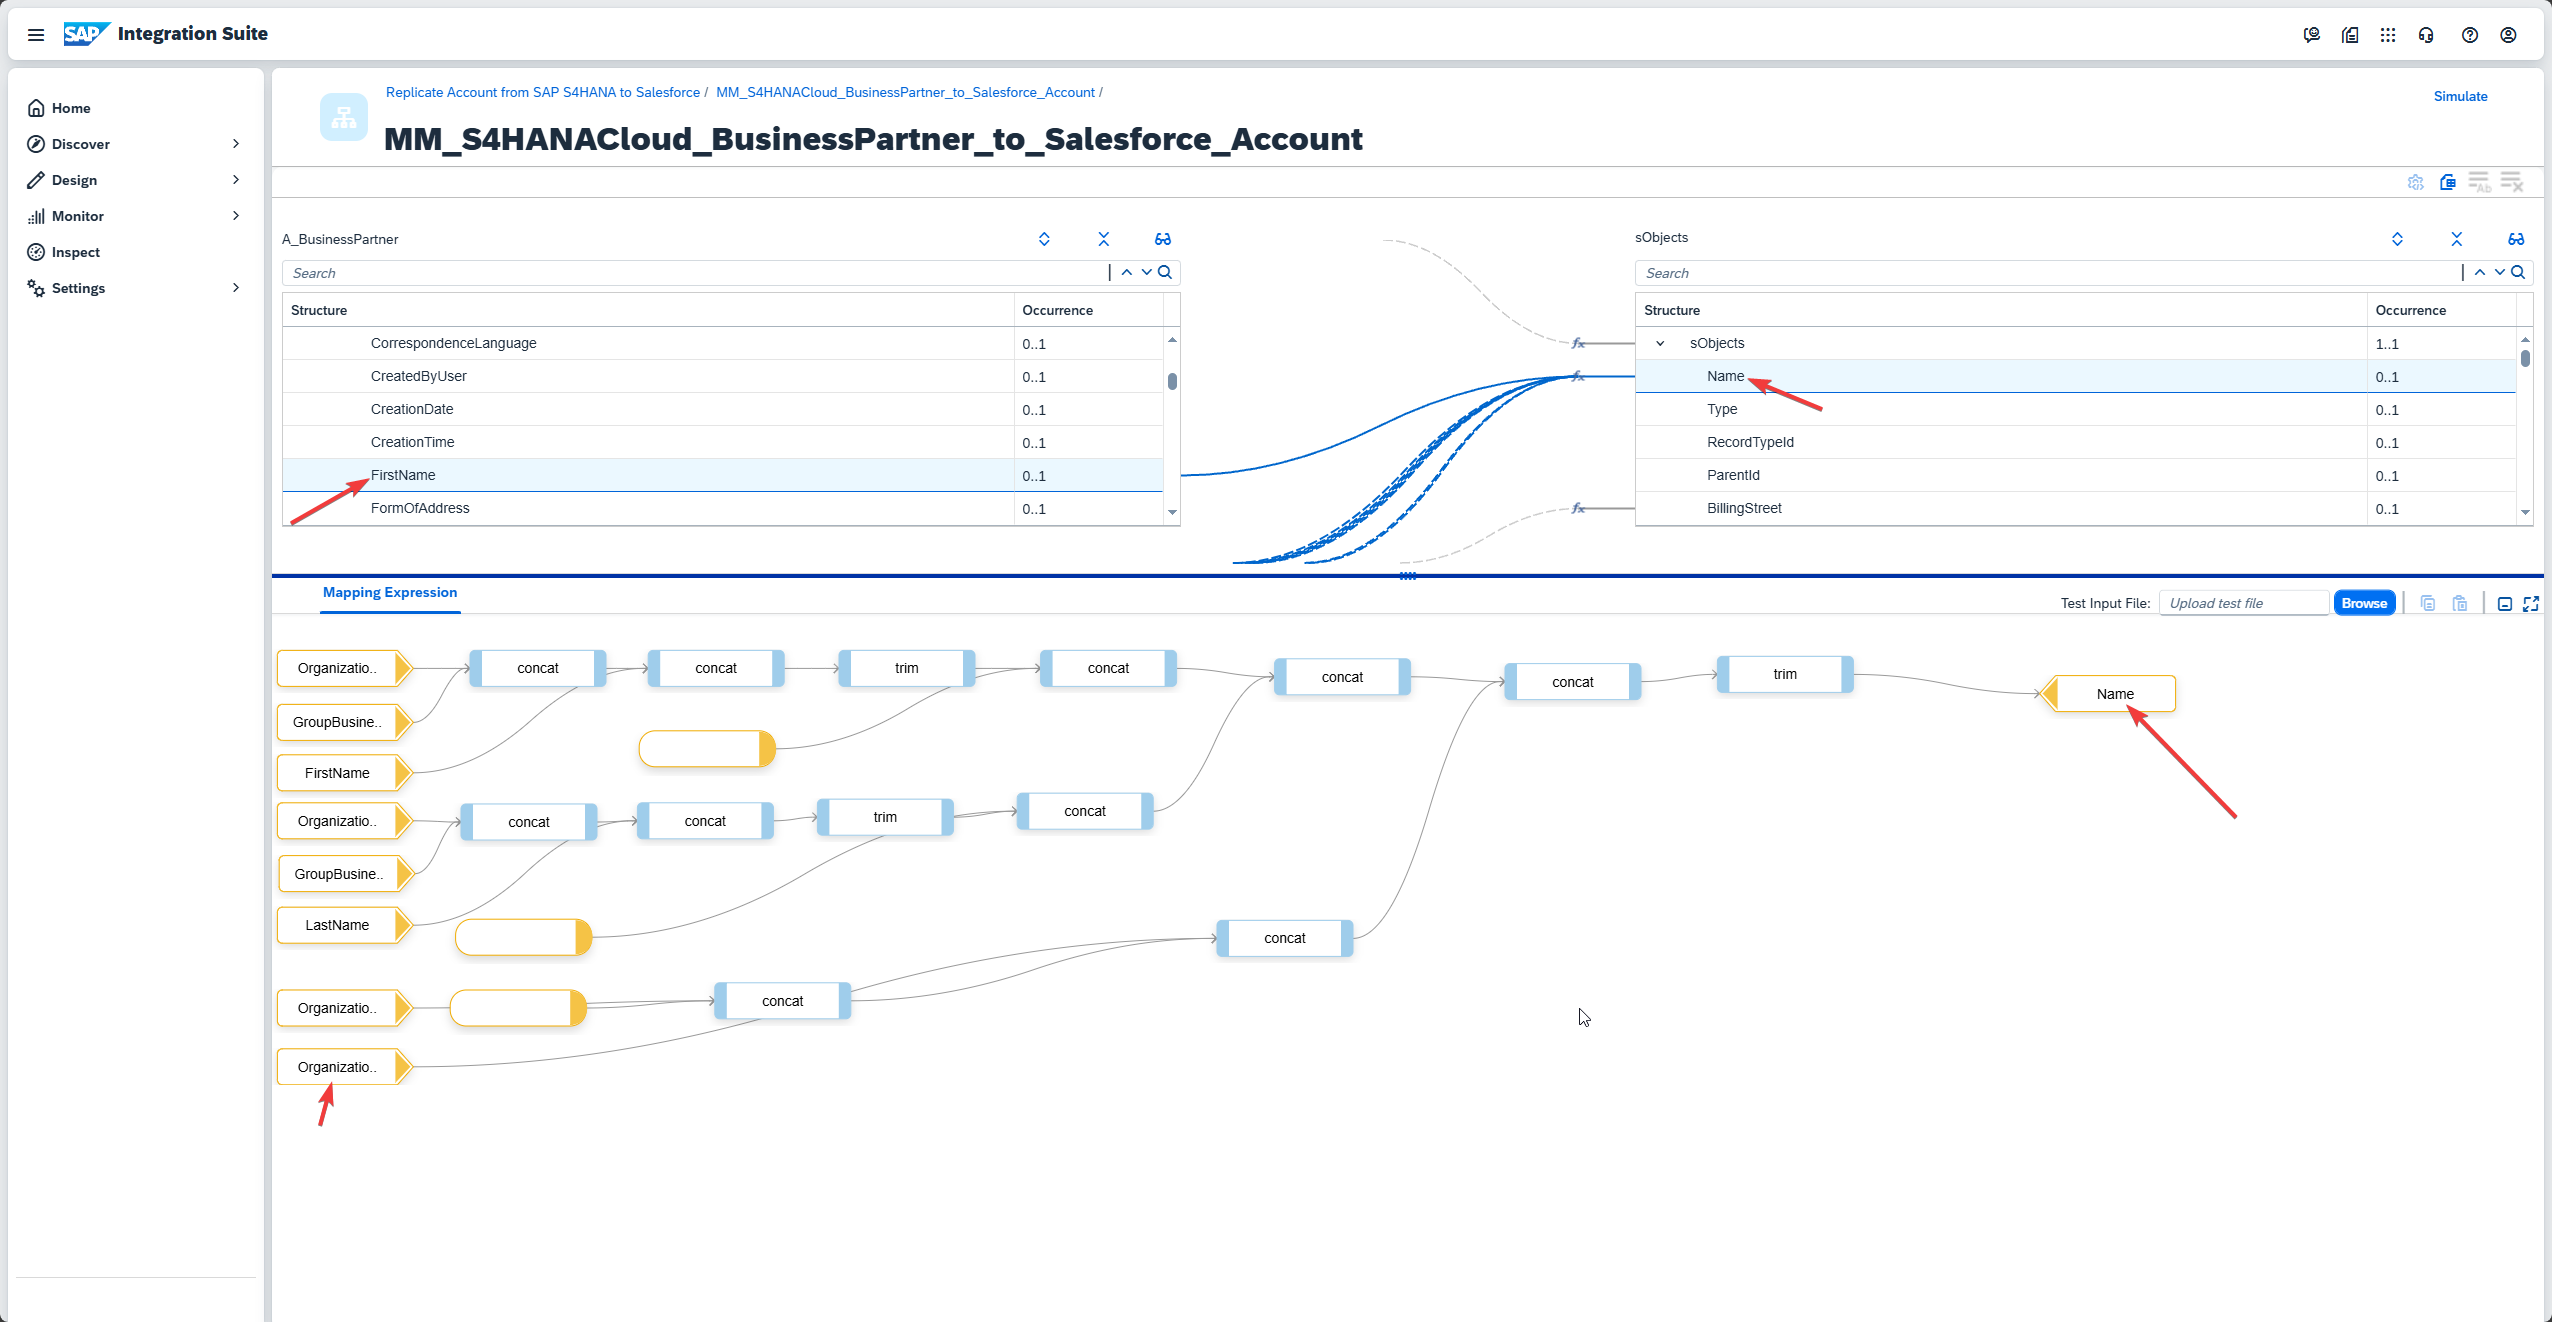
\includegraphics[width=0.8\textwidth]{Chapter5/Pictures/Map_comp.png}}
    \caption{Mapping Configuration in SAP BTP Integration Suite}
    
    \end{figure}

For example, SAP S/4HANA stores business partner names in multiple fields such as \texttt{Name1}, \texttt{Name2}, \texttt{Name3}, and \texttt{Name4}, while Salesforce represents the account name in a single field. This structural difference requires custom logic in the iFlow to concatenate and properly format the name fields before transferring the data to Salesforce. A screenshot illustrating this mapping challenge is provided below.



Such discrepancies necessitate additional transformation logic, increasing the complexity of iFlow development. Any misalignment in these mappings can result in data loss, formatting issues, or incorrect updates in Salesforce. Future improvements could focus on predefined mapping templates or automated field transformations to minimize manual effort.

\subsection{Limited Error Message Clarity}
Another critical limitation in the current development is the lack of detailed and actionable error messages in SAP CPI logs. The system often returns generic error responses, making it difficult to pinpoint the exact cause of failure.

A practical example of this issue was encountered in Section 5.2, where expired OAuth credentials were deliberately used to simulate an authentication failure. Instead of a clear authentication error message, SAP CPI returned a vague error log entry:

\begin{quote}
\texttt{Error Details org.apache.camel.CamelException:}
\end{quote}

Such non-descriptive error messages hinder troubleshooting and increase the time required for debugging. Developers must manually investigate multiple log files, cross-check API responses, and perform trial-and-error debugging to identify root causes. A potential improvement would be enhancing error verbosity in SAP CPI by enabling detailed logging or implementing structured error-handling mechanisms.

\subsection{Trial Account Restrictions and Licensing Issues}
A significant limitation in adopting this integration framework is the lack of access to the SAP CPI Integration Suite in trial accounts. Currently, SAP restricts trial users from connecting SAP S/4HANA with external applications via CPI. This creates several challenges:

\begin{itemize}
    \item Organizations must purchase a licensed SAP CPI instance before testing whether the solution fits their business needs.
    \item Without a trial version, developers cannot validate their integration scenarios without financial investment.
    \item Users exploring SAP CPI for learning or proof-of-concept purposes are unable to perform real-world testing.
\end{itemize}

The absence of trial access significantly impacts small businesses or teams evaluating SAP solutions, as they must commit to licensing costs upfront. A potential resolution could be providing limited trial access with connectivity to sandbox environments, allowing users to experiment with CPI before making financial commitments.

The current development of SAP CPI integration with Salesforce presents key challenges in field mapping, error handling, and licensing restrictions. Addressing these limitations requires enhanced mapping automation, more detailed error logs, and improved access to trial environments. Future enhancements in these areas would make the integration process more efficient and accessible for businesses looking to implement seamless data synchronization between SAP S/4HANA and Salesforce.


%=== END OF CHAPTER FIVE ===
\newpage
